\section{Machine Learning: Window approach}
\label{mlwindow}

The goal of this module is to product triples from sentences and be an alternative to the grammatical approach.

We used machine learning algorithms in order to produce triples from scratch, without any grammatical library like \Stanford. Our work is mainly based on the paper \cite{collobert}.

Motivations come from three points:
\begin{itemize}
\item Because triples are linked to the semantic of the sentence, and not directly from the grammar, we could expect that avoid grammatical tools can be a good idea.
\item It has been shown that a machine learning approach can produce, for a large panel of different NLP problems, very good solutions, closed to \textit{state of the art} algorithms \cite{collobert}.
\item Grammatical approaches fail on keyword sentences, like "Barack Obama birth date" because this kind of sentences does not respect the syntax of English.
\end{itemize}

Due to the restricted amount of time, we emphasis on keywords questions (keywords questions can not be analysed with grammatical tools) and we limit ourself to a restricted version of the data model:
\begin{itemize}
\item Only one level of depth: for example the sentence "What is the birth date of the president of the United States?" will be converted to the triple: (president of the United States, birth date, ?).
\item We do not support other kinds of connectors such as \texttt{first}, \texttt{sort}, etc.
\end{itemize}

We use a look-up table and a window approach neural network as explained below. The complete package\footnote{\url{https://github.com/ProjetPP/PPP-NLP-ML-standalone/}} was written in Python 3. We use the scikit-learn library, NumPy and NLTK as external tool.

Our algorithm can be described with three components: the look up table, the window approach, and the classifier.

\subsubsection{Look-up table}

The look-up table is a dictionary that associates to each word $w$ a vector $V_w \in \mathbb{R}^n$, where n is the number of parameters used to encode a word (we used $n=25$).
If two English words $w_1$ and $w_2$ are synonymous, then $||w_1-w_2||_2$ is small.

The construction of the look-up table is described in \cite{collobert} and used unsupervised machine learning techniques.
We used the pre-computed look-up table found here: \url{http://metaoptimize.com/projects/wordreprs/}

We also add one parameter to know if the word starts with a uppercase letter or not. Finally, words are embedded in vectors of dimension 26. 

\subsubsection{Window approach}

We use a window (as explain in \cite{collobert}) that focuses on one word to perform the classification. For instance, if the sentence is "What is the birth date of the president of France?", and the word to classify is "date", for a window size of 7, the window is: "is the birth \textbf{date} of the president".

We use this window because classifier algorithms usually work with a fixed number of input parameters. 

The window size is a meta parameter to choose. This window has to be large enough that we can decide in the context of the window in which category a word is. We used a window of size 9.

\subsubsection{The classifier}

If the question is "What is the birth date of the president of France?", and the focus of the window approach is on the word \textbf{date}, then the goal is to classify the word \textbf{date} into one of these four categories: \textit{subject}, \textit{predicate}, \textit{object}, \textit{to forget}.

The classification of each word of the sentence into these four categories finally gives us the desired triple.

The principle of the complete algorithm can be summarize in the figure ~\ref{sandalone:model}.

\begin{figure}[!ht]
  \centering
  \caption{The architecture of the algorithm, as described in \cite{collobert}}
  \label{sandalone:model}
    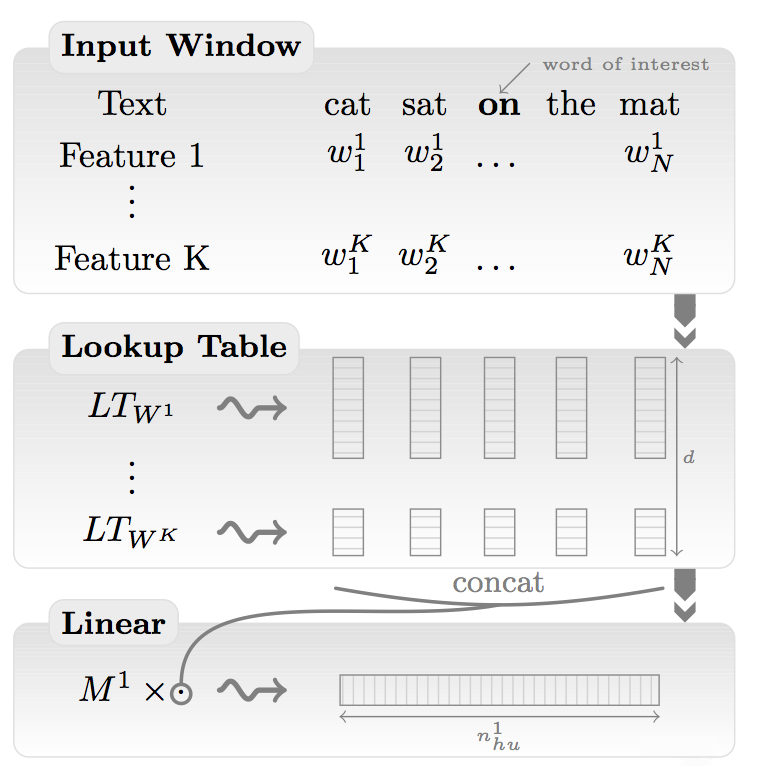
\includegraphics[scale=0.5]{../NLP-standalone-images/model.png}
\end{figure}

Because we have a small data set of annotated questions (see below), we use a linear model: a linear model has the advantage to have few parameters.
For example with a window approach of size 9 and words embedded in vectors of dimension 26,  this gives us $26\times 9\times 4 = 936$ parameters to learn.

In a first time we implemented our own linear classifier, but to improve the execution time, we finally use the \textit{LDA} classifier from the library scikit-learn. Few seconds of computation are now needed to train successfully the model.

\subsection{Data set}

Because we used supervised algorithms, we need a data set of annotated questions, in order to learn our model.
This data set was mostly built manually, because we did not find on the internet a data set that directly answering the problem of triple extraction.
Build this data set is a fastidious work. Currently our data set is composed of 300 questions.
We also wrote a script that generate keywords questions. This script gives us 500 keywords questions and makes the module specialized on keywords questions.

We now denote $\mathcal{D}_{GC}$ (for \textit{Data set Grammatically Correct}) the data set of grammatically correct questions, $\mathcal{D}_{kw}$ for the data set of generated keywords questions and $\mathcal{D}_A = \mathcal{D}_{GC} \cup  \mathcal{D}_{KW}$ the complete data set.

\subsection{Results}

In this basic configuration, we can measure the accuracy of our algorithm, defined as the ratio of correctly classified words, for a specified data set.

Our methodology is the following: for a specified data set $\mathcal{D} \in \{\mathcal{D}_A, \mathcal{D}_{GC}, \mathcal{D}_{KW}\}$ we split $\mathcal{D}$ in two parts: the training set and the test set (90% of the data is for the training set and 10% for the testing set). We learn our classifier with the training set and then evaluate it on the test set.
\todo{il y a une partie commentée ici, je sais pas si c'est volontaire}

\textbf{Remark}: to compute the accuracy of one variant of our algorithm we split the data set into testing and training set randomly, and we restart an experience 50 times. This makes us sure of the precision of the estimated accuracy.

\begin{center}
\begin{tabular}{|l|c|r|}
  \hline
  Data set &  Testing accuracy  & Training accuracy \\
  \hline
  $\mathcal{D}_{GC}$ &  $75\%$& $81\%$  \\
  $\mathcal{D}_{KW}$ & $98\%$ & $98.3\%$ \\
  $\mathcal{D}_{A}$    & $83\%$ & $86\%$ \\
  \hline
\end{tabular}
\end{center}

We can conclude that this version of the algorithm is excellent for keyword questions, and not really good for grammatically correct questions.

\subsubsection{Bias vs Variance test}

We can plot the \textit{Bias versus Variance} curves:

\begin{figure}[!ht]
  \centering
  \caption{Bias vs Variance curve for the data set  $\mathcal{D}_{GC}$}
  \label{sandalone:bias_vs_variance_1}
    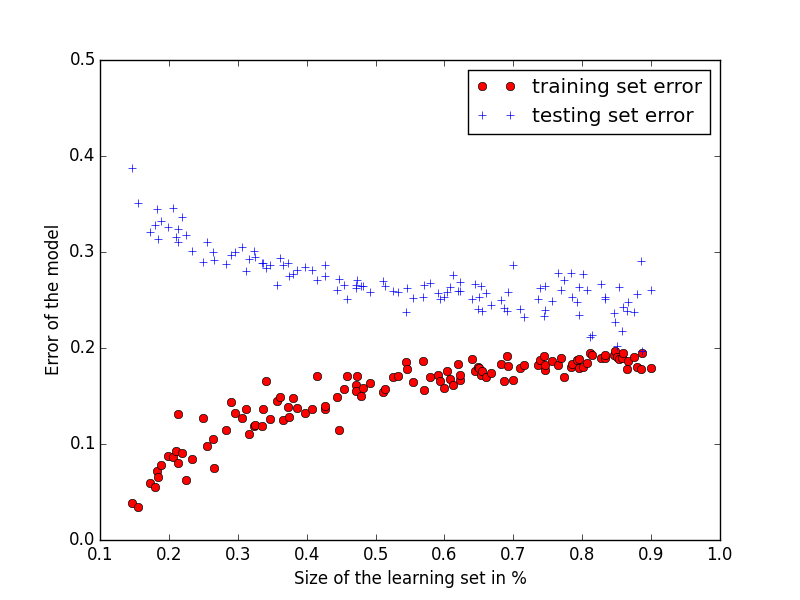
\includegraphics[scale=0.5]{../NLP-standalone-images/BiasVsVarianceD_GC.png}
\end{figure}

\begin{figure}[!ht]
  \centering
  \caption{Bias vs Variance curve for the data set  $\mathcal{D}_{KW}$}
  \label{sandalone:bias_vs_variance_2}
    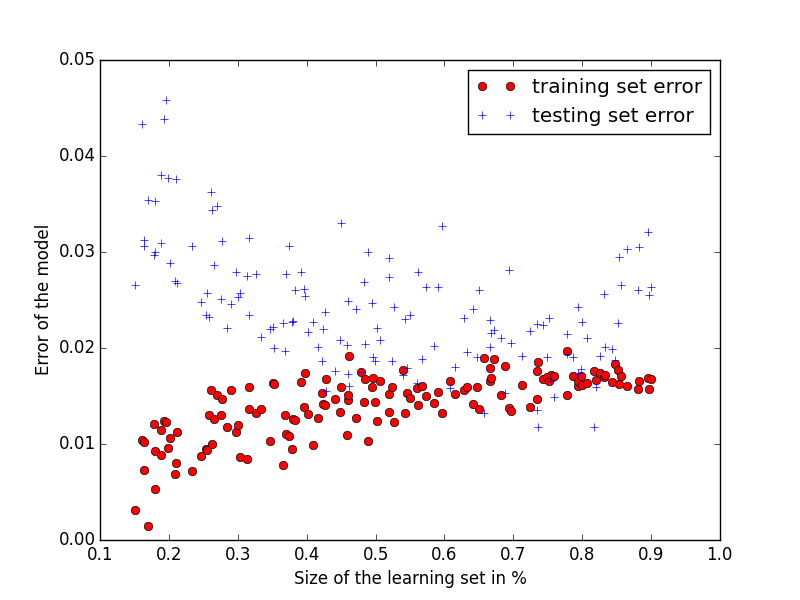
\includegraphics[scale=0.5]{../NLP-standalone-images/BiasVsVarianceD_KW.png}
\end{figure}

\begin{figure}[!ht]
  \centering
  \caption{Bias vs Variance curve for the data set  $\mathcal{D}_{A}$ }
  \label{sandalone:bias_vs_variance_3}
    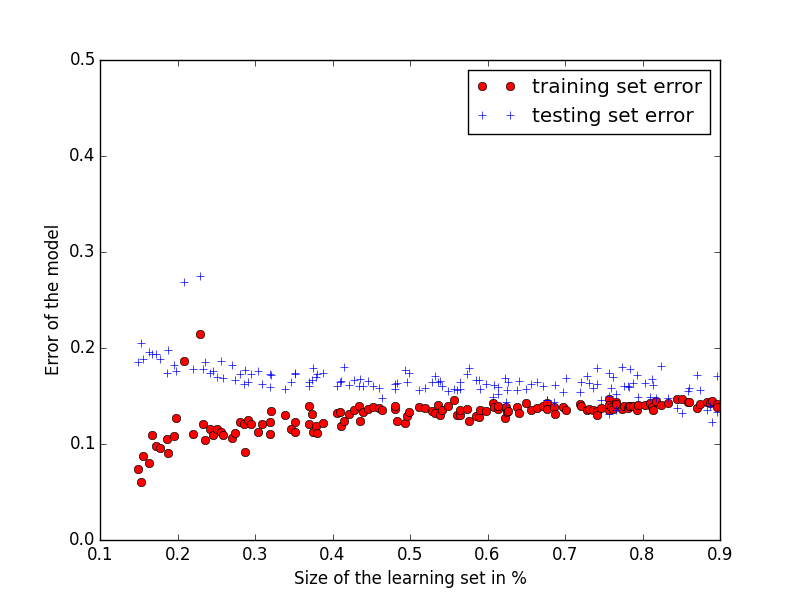
\includegraphics[scale=0.5]{../NLP-standalone-images/BiasVsVarianceD_A.png}
\end{figure}

These curves show us that there is a small gap between the two performances curves for the data set $\mathcal{D}_{GC}$: the data set of grammatically correct questions is too small to learn correctly the model.

However, when we add the keyword questions, the gap disappears: the model is learned correctly and the performances are good.

\subsection{Improvements of the algorithm}

\subsubsection{POS TAG features}

In order to help the classifier, we added POS TAG features: each word of the sentence is tagged with a grammatical tag (VERB, NOUN, PRON, ADJ, ...)

We use the NLTK pos tagger to do that. With such a tag, a word is encoded as a vector of dimension $26+11 = 37$.

This new feature helps improve the accuracy of the algorithm of few percents:

\begin{center}
\begin{tabular}{|l|c|r|}
  \hline
  Data set & Testing accuracy  without POS TAG & Testing accuracy  with POS TAG \\
  \hline
  $\mathcal{D}_{GC}$ &  $75\%$& $77.2\%$  \\
  $\mathcal{D}_{KW}$ & $98\%$ & $98.9\%$ \\
  $\mathcal{D}_{A}$    & $83\%$ & $86\%$ \\
  \hline
\end{tabular}
\end{center}


\subsection{Conclusion}

The initial goal was to make a concurrent of the grammatical approach to transform English questions into the data model. Due to the limited amount of time, we did not succeed to improve sufficiently the accuracy of the classifier to make this approach as good as the grammatical approach.

We decided then to focus on keywords questions, which are very important for a framework of question answering. For this task, with a good data set of annotated keywords questions, this algorithm is really efficient.

